\documentclass[a4paper,12pt]{article}
%%% Работа с русским языком % для pdfLatex
\usepackage{cmap}					% поиск в~PDF
\usepackage{mathtext} 				% русские буквы в~фомулах
\usepackage[T2A]{fontenc}			% кодировка
\usepackage[utf8]{inputenc}			% кодировка исходного текста
\usepackage[english,russian]{babel}	% локализация и переносы
\usepackage{indentfirst} 			% отступ 1 абзаца

%%% Работа с русским языком % для XeLatex
%\usepackage[english,russian]{babel}   %% загружает пакет многоязыковой вёрстки
%\usepackage{fontspec}      %% подготавливает загрузку шрифтов Open Type, True Type и др.
%\defaultfontfeatures{Ligatures={TeX},Renderer=Basic}  %% свойства шрифтов по умолчанию
%\setmainfont[Ligatures={TeX,Historic}]{Times New Roman} %% задаёт основной шрифт документа
%\setsansfont{Comic Sans MS}                    %% задаёт шрифт без засечек
%\setmonofont{Courier New}
%\usepackage{indentfirst}
%\frenchspacing

%%% Дополнительная работа с математикой
\usepackage{amsfonts,amssymb,amsthm,mathtools}
\usepackage{amsmath}
\usepackage{icomma} % "Умная" запятая: $0,2$ --- число, $0, 2$ --- перечисление
\usepackage{upgreek}

%% Номера формул
%\mathtoolsset{showonlyrefs=true} % Показывать номера только у тех формул, на которые есть \eqref{} в~тексте.

%%% Страница
\usepackage{extsizes} % Возможность сделать 14-й шрифт

%% Шрифты
\usepackage{euscript}	 % Шрифт Евклид
\usepackage{mathrsfs} % Красивый матшрифт

%% Свои команды
\DeclareMathOperator{\sgn}{\mathop{sgn}} % создание новой конанды \sgn (типо как \sin)
\usepackage{csquotes} % ещё одна штука для цитат
\newcommand{\pd}[2]{\ensuremath{\cfrac{\partial #1}{\partial #2}}} % частная производная
\newcommand{\abs}[1]{\ensuremath{\left|#1\right|}} % модуль
\renewcommand{\phi}{\ensuremath{\varphi}} % греческая фи
\newcommand{\pogk}[1]{\!\left(\cfrac{\sigma_{#1}}{#1}\right)^{\!\!\!2}\!} % для погрешностей

% Ссылки
\usepackage{color} % подключить пакет color
% выбрать цвета
\definecolor{BlueGreen}{RGB}{49,152,255}
\definecolor{Violet}{RGB}{120,80,120}
% назначить цвета при подключении hyperref
\usepackage[unicode, colorlinks, urlcolor=blue, linkcolor=blue, pagecolor=blue, citecolor=blue]{hyperref} %синие ссылки
%\usepackage[unicode, colorlinks, urlcolor=black, linkcolor=black, pagecolor=black, citecolor=black]{hyperref} % для печати (отключить верхний!)


%% Перенос знаков в~формулах (по Львовскому)
\newcommand*{\hm}[1]{#1\nobreak\discretionary{}
	{\hbox{$\mathsurround=0pt #1$}}{}}

%%% Работа с картинками
\usepackage{graphicx}  % Для вставки рисунков
\graphicspath{{images/}{images2/}}  % папки с картинками
\setlength\fboxsep{3pt} % Отступ рамки \fbox{} от рисунка
\setlength\fboxrule{1pt} % Толщина линий рамки \fbox{}
\usepackage{wrapfig} % Обтекание рисунков и таблиц текстом
\usepackage{multicol}

%%% Работа с таблицами
\usepackage{array,tabularx,tabulary,booktabs} % Дополнительная работа с таблицами
\usepackage{longtable}  % Длинные таблицы
\usepackage{multirow} % Слияние строк в~таблице
\usepackage{caption}
\captionsetup{labelsep=period, labelfont=bf}

%%% Оформление
\usepackage{indentfirst} % Красная строка
%\setlength{\parskip}{0.3cm} % отступы между абзацами
%%% Название разделов
\usepackage{titlesec}
\titlelabel{\thetitle.\quad}
\renewcommand{\figurename}{\textbf{Рис.}}		%Чтобы вместо figure под рисунками писал "рис"
\renewcommand{\tablename}{\textbf{Таблица}}		%Чтобы вместо table над таблицами писал Таблица

%%% Теоремы
\theoremstyle{plain} % Это стиль по умолчанию, его можно не переопределять.
\newtheorem{theorem}{Теорема}[section]
\newtheorem{proposition}[theorem]{Утверждение}

\theoremstyle{definition} % "Определение"
\newtheorem{definition}{Определение}[section]
\newtheorem{corollary}{Следствие}[theorem]
\newtheorem{problem}{Задача}[section]

\theoremstyle{remark} % "Примечание"
\newtheorem*{nonum}{Решение}
\newtheorem{zamech}{Замечание}[theorem]

%%% Правильные мат. символы для русского языка
\renewcommand{\epsilon}{\ensuremath{\varepsilon}}
\renewcommand{\phi}{\ensuremath{\varphi}}
\renewcommand{\kappa}{\ensuremath{\varkappa}}
\renewcommand{\le}{\ensuremath{\leqslant}}
\renewcommand{\leq}{\ensuremath{\leqslant}}
\renewcommand{\ge}{\ensuremath{\geqslant}}
\renewcommand{\geq}{\ensuremath{\geqslant}}
\renewcommand{\emptyset}{\varnothing}

\usepackage{bm} %жирный греческий шрифт
%\usepackage{ulem}

\graphicspath{{images}}
\title{Laba 1.4.2}
\author{Георгий Демьянов}
\date{November 2016}
\usepackage[left=1.27cm,right=1.27cm,top=1.27cm,bottom=2cm]{geometry}

\begin{document} 
\begin{titlepage}
\begin{center} 
\large Московский физико-технический институт\\
Факультет молекулярной и химической физики\\
\vspace{7cm}
\huge Лабораторная работа №1.4.2\\
\textbf{\Large <<Определение ускорения свободного падения при помощи оборотного маятника>>}\\
\end{center} 

\vspace{7.5cm}
{\par \raggedleft \large \emph{Выполнил:}\\ студент 1 курса\\ 642 группы ФМХФ\\ Демьянов Георгий\\ Сергеевич \par}
\begin{center}
\vfill Москва 2016
\end{center}
\end{titlepage}

\newpage

\textbf{\emph{Цель работы:}} определить величину ускорения свободного падения.

\textbf{\emph{Оборудование:}} оборотный маятник, счетчик числа колебаний, секундомер, штангенциркуль с пределом измерений 1 м.

\textbf{\section{Теоретическое введение}}

Ускорение свободного падения, которое вблизи поверхности обычно обозначают $g$, определяется массой тела $m$ и силой $F$, действующей на тело,
\begin{center}
	\vspace{-20pt}
	\begin{equation}
	\vec g = \cfrac{\vec F}{m}.
	\label{g_1}
	\end{equation}
	\vspace{-20pt}
\end{center}

Ускорение свободного падения можно измерить с помощью физического маятника. Период колебаний физического маятника определяется формулой:
\begin{center}
	\vspace{-20pt}
	\begin{equation}
	T=2\pi \sqrt{\cfrac{I}{mga}}.
	\label{T}
	\end{equation}
	\vspace{-20pt}
\end{center}
Здесь $I$ - момент инерции маятника относительно оси качения, $m$ - масса маятника, $a$ - расстояние от центра масс до оси качения.

Массу маятника и период колебаний можно измерить с очень высокой точностью, но точно измерить момент инерции не удается. Указанного недостатка лишен метод оборотного маятника, который позволяет исключить момент инерции из расчетной формулы для $g$.

Метод оборотного маятника основан на том, что период колебаний физического маятника не изменяется при перемещении оси качаний в центр качаний, т.е. в точку, отстоящую от оси качаний на расстояние, равное приведенной длине маятника, и лежащую на одной прямой с точкой подвеса и центром масс маятника.

Применяемый в настоящей работе оборотный маятник (рис. \ref{img_1}) состоит из стальной пластины, на которой укреплены две однородные призмы П$_1$ и П$_2$. Период колебаний маятника можно менять при помощи подвижных грузов Г$_1$, Г$_2$ и Г$_3$.

Если нам удалось найти такое положение грузов, при котором периоды колебаний маятника $T_1$ и $T_2$  на призмах  П$_1$ и П$_2$ совпадают, то справедливо:
\begin{center}
	\vspace{-20pt}
	\begin{equation}
	T_1=T_2=T=2\pi \sqrt{\cfrac{I_1}{mga_1}}=2\pi \sqrt{\cfrac{I_2}{mga_2}},
	\label{T_1=T_2}
	\end{equation}
	\vspace{-20pt}
\end{center}
где $a_1$ и $a_2$ - расстояния от центра массы маятника до призм П$_1$ и П$_2$.

Условием этого является равенство приведенных длин, т.е. равенство величин $\cfrac{I_1}{ma_1}$ и $\cfrac{I_2}{ma_2}$. По теореме Гюйгенса-Штейнера:
\begin{center}
	\vspace{-20pt}
	\begin{equation}
	I_1=I_0+ma_{2}^2, I_2=I_0+ma_{2}^2,
	\label{I_1}
	\end{equation}
	\vspace{-20pt}
\end{center}
где $I_0$ - момент инерции маятника относительно оси, проходящей через его центр масс. Исключая из \eqref{T_1=T_2} и \eqref{I_1} $I_0$ и $m$, получим формулу для определения $g$:
\begin{center}
	\vspace{-20pt}
	\begin{equation}
	g = \cfrac{4\pi^2}{T^2}(a_1+a_2) = 4\pi^2 \cfrac{L}{T^2},
	\label{g}
	\end{equation}
	\vspace{-20pt}
\end{center}
Здесь $L=a_1+a_2$ — расстояние между призмами П$_1$ и П$_2$ (причем $a_1 \neq a_2$), которое легко может быть измерено с высокой точностью ($0.1$ мм) при помощи большого штангенциркуля.

При выводе формулы \eqref{g} мы полагали, что $T_1=T_2$, что на практике невозможно. Тогда
$$
T_i=2\pi \sqrt{\cfrac{I_i}{mga_i}}, i = 1, 2,
$$
откуда получим формулу:
\begin{center}
	\vspace{-20pt}
	\begin{equation}
	\fbox{
	$g = 4 \pi^2 \cfrac{a_1^2-a_2^2}{a_1 T_1^2-a_2 T_2^2} = 4 \pi^2 \cfrac{L}{T_0^2}$},
	\label{g_k}
	\end{equation}
	\vspace{-20pt}
\end{center}
где
\begin{center}
	\vspace{-20pt}
	\begin{equation}
	\fbox{
	$T_0^2=T_2^2+\cfrac{L-a_2}{L-2a_2}(T_1^2-T_2^2)$}.
	\label{T_0}
	\end{equation}
	\vspace{-20pt}
\end{center}
Погрешность $g$ может найдена из \eqref{g_k}:
\begin{center}
	\vspace{-20pt}
	\begin{equation}
	\fbox{
	$\cfrac{\sigma_g}{g} = \sqrt{\left(\cfrac{\sigma_L}{L}\right)^2 + 4 \left(\cfrac{\sigma_{T_0}}{T_0} \right)^2}$}.
	\label{error_g}
	\end{equation}
	\vspace{-20pt}
\end{center}
Погрешность $\sigma_{T_0}$ найдем по формуле:
\begin{center}
	\vspace{-20pt}
	\begin{equation}
	\fbox{
	$\sigma_{T_0^2}^2=\left| \cfrac{\partial(T_0^2)}{\partial(T_2^2)} \right|^2 \sigma_{T_2^2}^2+\left| \cfrac{\partial(T_0^2)}{\partial(L)} \right|^2 \sigma_{L}^2+\left| \cfrac{\partial(T_0^2)}{\partial(a_2)} \right|^2 \sigma_{a_2}^2+\left| \cfrac{\partial(T_0^2)}{\partial(T_1^2)} \right|^2 \sigma_{T_1^2}^2$},
	\label{error_T_0}
	\end{equation}
	\vspace{-20pt}
\end{center}
где
\begin{center}
	\vspace{-20pt}
	\begin{equation}
	\left| \cfrac{\partial(T_0^2)}{\partial(T_2^2)} \right|=\left|\cfrac{a_2}{2a_2-L}\right|
	\label{10}
	\end{equation}
	\vspace{-20pt}
\end{center}
\begin{center}
	\vspace{-20pt}
	\begin{equation}
	\left| \cfrac{\partial(T_0^2)}{\partial(L)} \right| = \left|\cfrac{T_2^2-T_1^2}{(L-2a_2)^2}\, a_2\right|
	\end{equation}
	\vspace{-20pt}
\end{center}
\begin{center}
	\vspace{-20pt}
	\begin{equation}
	\left| \cfrac{\partial(T_0^2)}{\partial(a_2)} \right| = \left|\cfrac{T_1^2-T_2^2}{(L-2a_2)^2}\, L\right|
	\end{equation}
	\vspace{-20pt}
\end{center}
\begin{center}
	\vspace{-20pt}
	\begin{equation}
	\left| \cfrac{\partial(T_0^2)}{\partial(T_1^2)} \right| = \left|\cfrac{L-a_2}{L-2a_2}\right|
	\label{13}
	\end{equation}
	\vspace{-20pt}
\end{center}
\begin{center}
	\vspace{-20pt}
	\begin{equation}
	\sigma_{T_2^2}=2 \sigma_{T_2} T_2
	\end{equation}
	\vspace{-20pt}
\end{center}
\begin{center}
	\vspace{-20pt}
	\begin{equation}
	\sigma_{T_1^2}=2\sigma_{T_1} T_1.
	\label{15}
	\end{equation}
	\vspace{-20pt}
\end{center}
А $\sigma_{T_0}$ найдем так:
\begin{center}
	\vspace{-20pt}
	\begin{equation}
	\sigma_{T_0^2}=2\sigma_{T_0} T_0 \Rightarrow \sigma_{T_0}=\cfrac{\sigma_{T_0^2}}{2T_0}.
	\end{equation}
	\vspace{-20pt}
\end{center}
Теоретические выкладки взяты из \cite{Gladun:PrakMech} - с. 252-256.

\newpage

\textbf{\section{Схема экспериментальной установки}}

Схема устройства оборотного маятника изображена на рис. \ref{img_1}. Расстояние $L$ между опорными призмами
П$_1$ и П$_2$ не меняется. Расстояния $a_1$ и $a_2$ можно менять, перемещая
грузы Г$_1$, Г$_2$ и Г$_3$.
Для определения числа колебаний используется счетчик, состоящий из осветителя, фотоэлемента и пересчетного устройства. Легкий
стержень, укрепленный на торце маятника, пересекает световой луч
дважды за период. Возникающие в фотоэлементе импульсы поступают
на пересчетный прибор. Если $n_1$ и $n_2$ - начальное и конечное значения показаний прибора за время наблюдения $t$, то измеренное число
периодов, очевидно, равно $N = \cfrac{n_2-n_1}{2}$, а период колебаний равен $T=\cfrac{t}{N}$. Время t измеряется секундомером, установленным
на пересчетном приборе. Для определения расстояний $a_1$ и $a_2$ маятник
снимают с консоли и располагают горизонтально на специальной подставке, имеющей острую грань. Перемещая маятник, нетрудно найти
положение центра масс. Расстояния от него до опорных призм и есть
искомые $a_1$ и $a_2$.

Описание установки взято из \cite{Gladun:PrakMech} - с. 257.
\begin{figure}[h]
	\vspace{1cm}
	\begin{center}
		\fbox{
			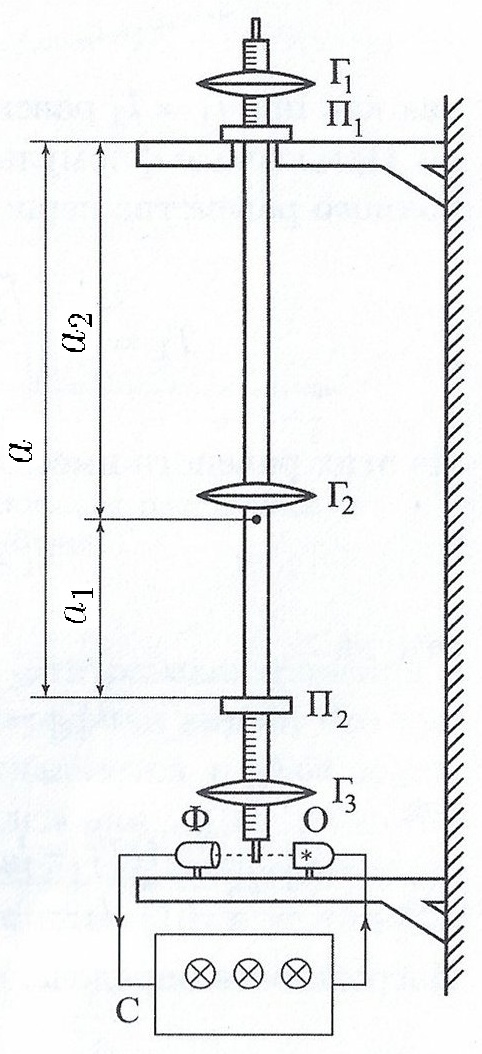
\includegraphics[width=0.34\textwidth]{SCAN0793.jpg}}
	\end{center}
	\caption{Схема экспериментальной установки}
	\label{img_1}
\end{figure}

\newpage
\textbf{\section{Обработка результатов}}

Проведя эксперимент, занесем полученные данные в таблицу:
\begin{table}[h!]
	\centering
	\caption{}
	\label{my-label}
	\begin{tabular}{|c|c|c|c|}
		\hline
		$t_1$, с & $t_2$, с & $L, 10^{-2}$ м & $a_2, 10^{-2}$ м \\ \hline
		$302.7 \pm 0.4$ & $300.6 \pm 0.4$ & $56.65 \pm 0.01$ & $20.9 \pm 0.1$ \\ \hline
	\end{tabular}
\end{table}

Тогда ($N=200$):
\begin{center}
	$T_1 = \cfrac{t_1}{N} = (1.514 \pm 0.002)\,$с
\end{center}
\begin{center}
	$T_2 = \cfrac{t_2}{N} = (1.503 \pm 0.002)\,$с.
\end{center}
Получим $T_0$ по формуле \eqref{T_0}:
\begin{center}
	$T_0=1.528\,$с.
\end{center}
Используя формулы \eqref{10}-\eqref{15}, определим значения:
$$\left| \cfrac{\partial(T_0^2)}{\partial(T_2^2)} \right|=1.41$$
$$\left| \cfrac{\partial(T_0^2)}{\partial(L)} \right|=0.31 \cfrac{\ \text{с}^2}{\text{м}}$$
$$\left|\, \cfrac{\partial(T_0^2)}{\partial(a_2)} \right|=0.85\, \cfrac{\text{с}^2}{\text{м}}$$
$$\left| \cfrac{\partial(T_0^2)}{\partial(T_1^2)} \right|=2.41$$
\begin{center}
	$\sigma_{T_1^2}=\sigma_{T_2^2} = 0.006\,\text{с}^2$,
\end{center}
откуда
\begin{center}
	\begin{equation}
	\sigma_{T_0^2} = 0.017\,\text{с}^{2} \Rightarrow \sigma_{T_0}= 0.006\,\text{с}.
	\end{equation}
\end{center}
В итоге:
\begin{center}
	\begin{equation}
	\fbox{
	$T_0 = (1.528 \pm 0.006)\, \text{с}$}.
	\end{equation}
\end{center}
\newpage
Интересно посмотреть на вклад слагаемых в погрешность $\sigma_{T_0^2}^2$ в формуле \eqref{error_T_0}:
\begin{table}[h!]
	\centering
	\caption{}
	\label{my-label_1}
	\begin{tabular}{|c|c|}
		\hline
		Частная производная $T_0^2$ по & Вклад в погрешность, \% \\ \hline
		$T_2^2$                        & 25.0821                 \\ \hline
		$L$                            & 0.0003                  \\ \hline
		$a_2$                          & 0.2546                  \\ \hline
		$T_1^2$                        & 74.6630                 \\ \hline
	\end{tabular}
\end{table}

Таким образом, видим, что слагаемыми, связанными с частными производными по $L$ и по $a_2$, можно пренебречь. Они не повлияют на конечное значение погрешности.

По формуле \eqref{g_k} найдем значение ускорения свободного падения $g$:
$$
g=9.56\, \cfrac{\text{м}}{\text{с}^2},
$$
а погрешность получим по формуле \eqref{error_g}:
$$
\sigma_g=0.07\, \cfrac{\text{м}}{\text{с}^2}.
$$
В итоге, получим:
\begin{center}
	\begin{equation}
	\fbox{
	$g=(9.56 \pm 0.07)\, \cfrac{\text{м}}{\text{с}^2}$}.
	\end{equation}
\end{center}

Сравним с табличным значением. Ускорение свободного падения на широте Москвы равно $g_0=9.82\, \cfrac{\text{м}}{\text{с}^2}$. Тогда полученное значение отличается от табличного на: $$\delta=\cfrac{|9.82-9.56|}{9.82} \cdot 100\%=2.65\%$$.
\newpage
\textbf{\section{Заключение}}

В данной работе мы измеряли ускорение свободного падения $g$ с помощью оборотного маятника. Были получены формулы: \eqref{g_k} и \eqref{T_0} для расчета значения $g$, \eqref{error_g} и  \eqref{error_T_0} - для погрешности измерений. Обработав экспериментальные данные по этим формулам, получили значение ускорения свободного падения $g=(9.56 \pm 0.07)\, \cfrac{\text{м}}{\text{с}^2}$, которое отличается от табличного значения на $2.65\%$.



\vspace{1cm}
\bibliography{mybibliography}
\bibliographystyle{gost705}

\end{document}